\chapter{Analyses}

\label{ch:analysis}

Before designing an educational product, it is important that the designer first acquaints himself with the extrinsic factors important to this product. In order to discover the important characteristics of these factors, \citeA{instructionaldesign} enlist three types of analyses to be conducted, together with steps for conducting them. These are an analysis of the context, encompassing the needs of the users, and the environmental characteristics, an analysis of the learner, and an analysis of the learning task. Although these analyses are more targeted towards instructional design, and therefore more focused on a specific group being taught specific content, these analyses will still provide relevant information for the design choices and the evaluation. However, the steps will be adjusted and generalised or even omitted in order to fit the design of the more generic learning tool. The information gathered in order to conduct these analyses mainly stems from meetings with one of the teachers. This might not be the most reliable source of information because of the lack of triangulation, and should therefore not be taken as insight in the curriculum of Dutch Literature courses in secondary education, but rather as context information relevant to the design.

\section{Analysis of the learning context}

As already stated in the \nameref{sec:intro_evaluation} section on page~\pageref{sec:intro_evaluation}, the evaluation of the flashmap system will be evaluated within the Dutch secondary school Stedelijk Lyceum, with students having to learn about the Renaissance genres in Dutch Literature. This context will be further investigated within this section, starting with the Needs Assessment \cite{instructionaldesign}. Because although the general needs for a flashmap system are already described in the \nameref{ch:problem}, it is still important to investigate the specific needs of the context where the programm will be implemented.

\subsection{Needs assessment}

According to \citeA{instructionaldesign}, the first step in a needs assessment is to assess whether there is a problem, and what the nature is of the problem (see figure~\ref{fig:needsassessment}, mostly to identify the problem, but also in order to assess whether the innovation model or the discrepancy model applies for determining the needs. The first step is to assess whether there really is a problem in order to establish the general need. During the meetings, the teacher did confirm the need for better retention and comprehension of the content, and indicated that most of the time the students only learned the night before the exam in order to get a high (enough) grade and consequently forget everything again. This is not only wasteful of the effort of learning, but also causes problems when the knowledge becomes relevant again in the next chapter. The cause of this problem therefore definitely lies within the learning process, and could possibly be improved by the use of a flashcard or flashmap system, so it can be concluded that there is indeed a problem caused by learning, and it is thereby useful to proceed with the next phase of the assessment. Finally, \citeA{instructionaldesign} finally state that if there already exists instruction for the relevant learning goals, since if so than one has to proceed by using the discrepancy model, and otherwise by using the innovation model. The new tool is only there to enhance the current learning process by adding an additional activity, rather than adding new learning goals to an empty space in the curriculum. Thereby, from an instructional perspecticve, the flashcard or flashmap system is only an improvement of the currently existing instructional activities rather than a new innovation, and therefore the discrepancy model will be used.

\begin{figure}
    \centering
    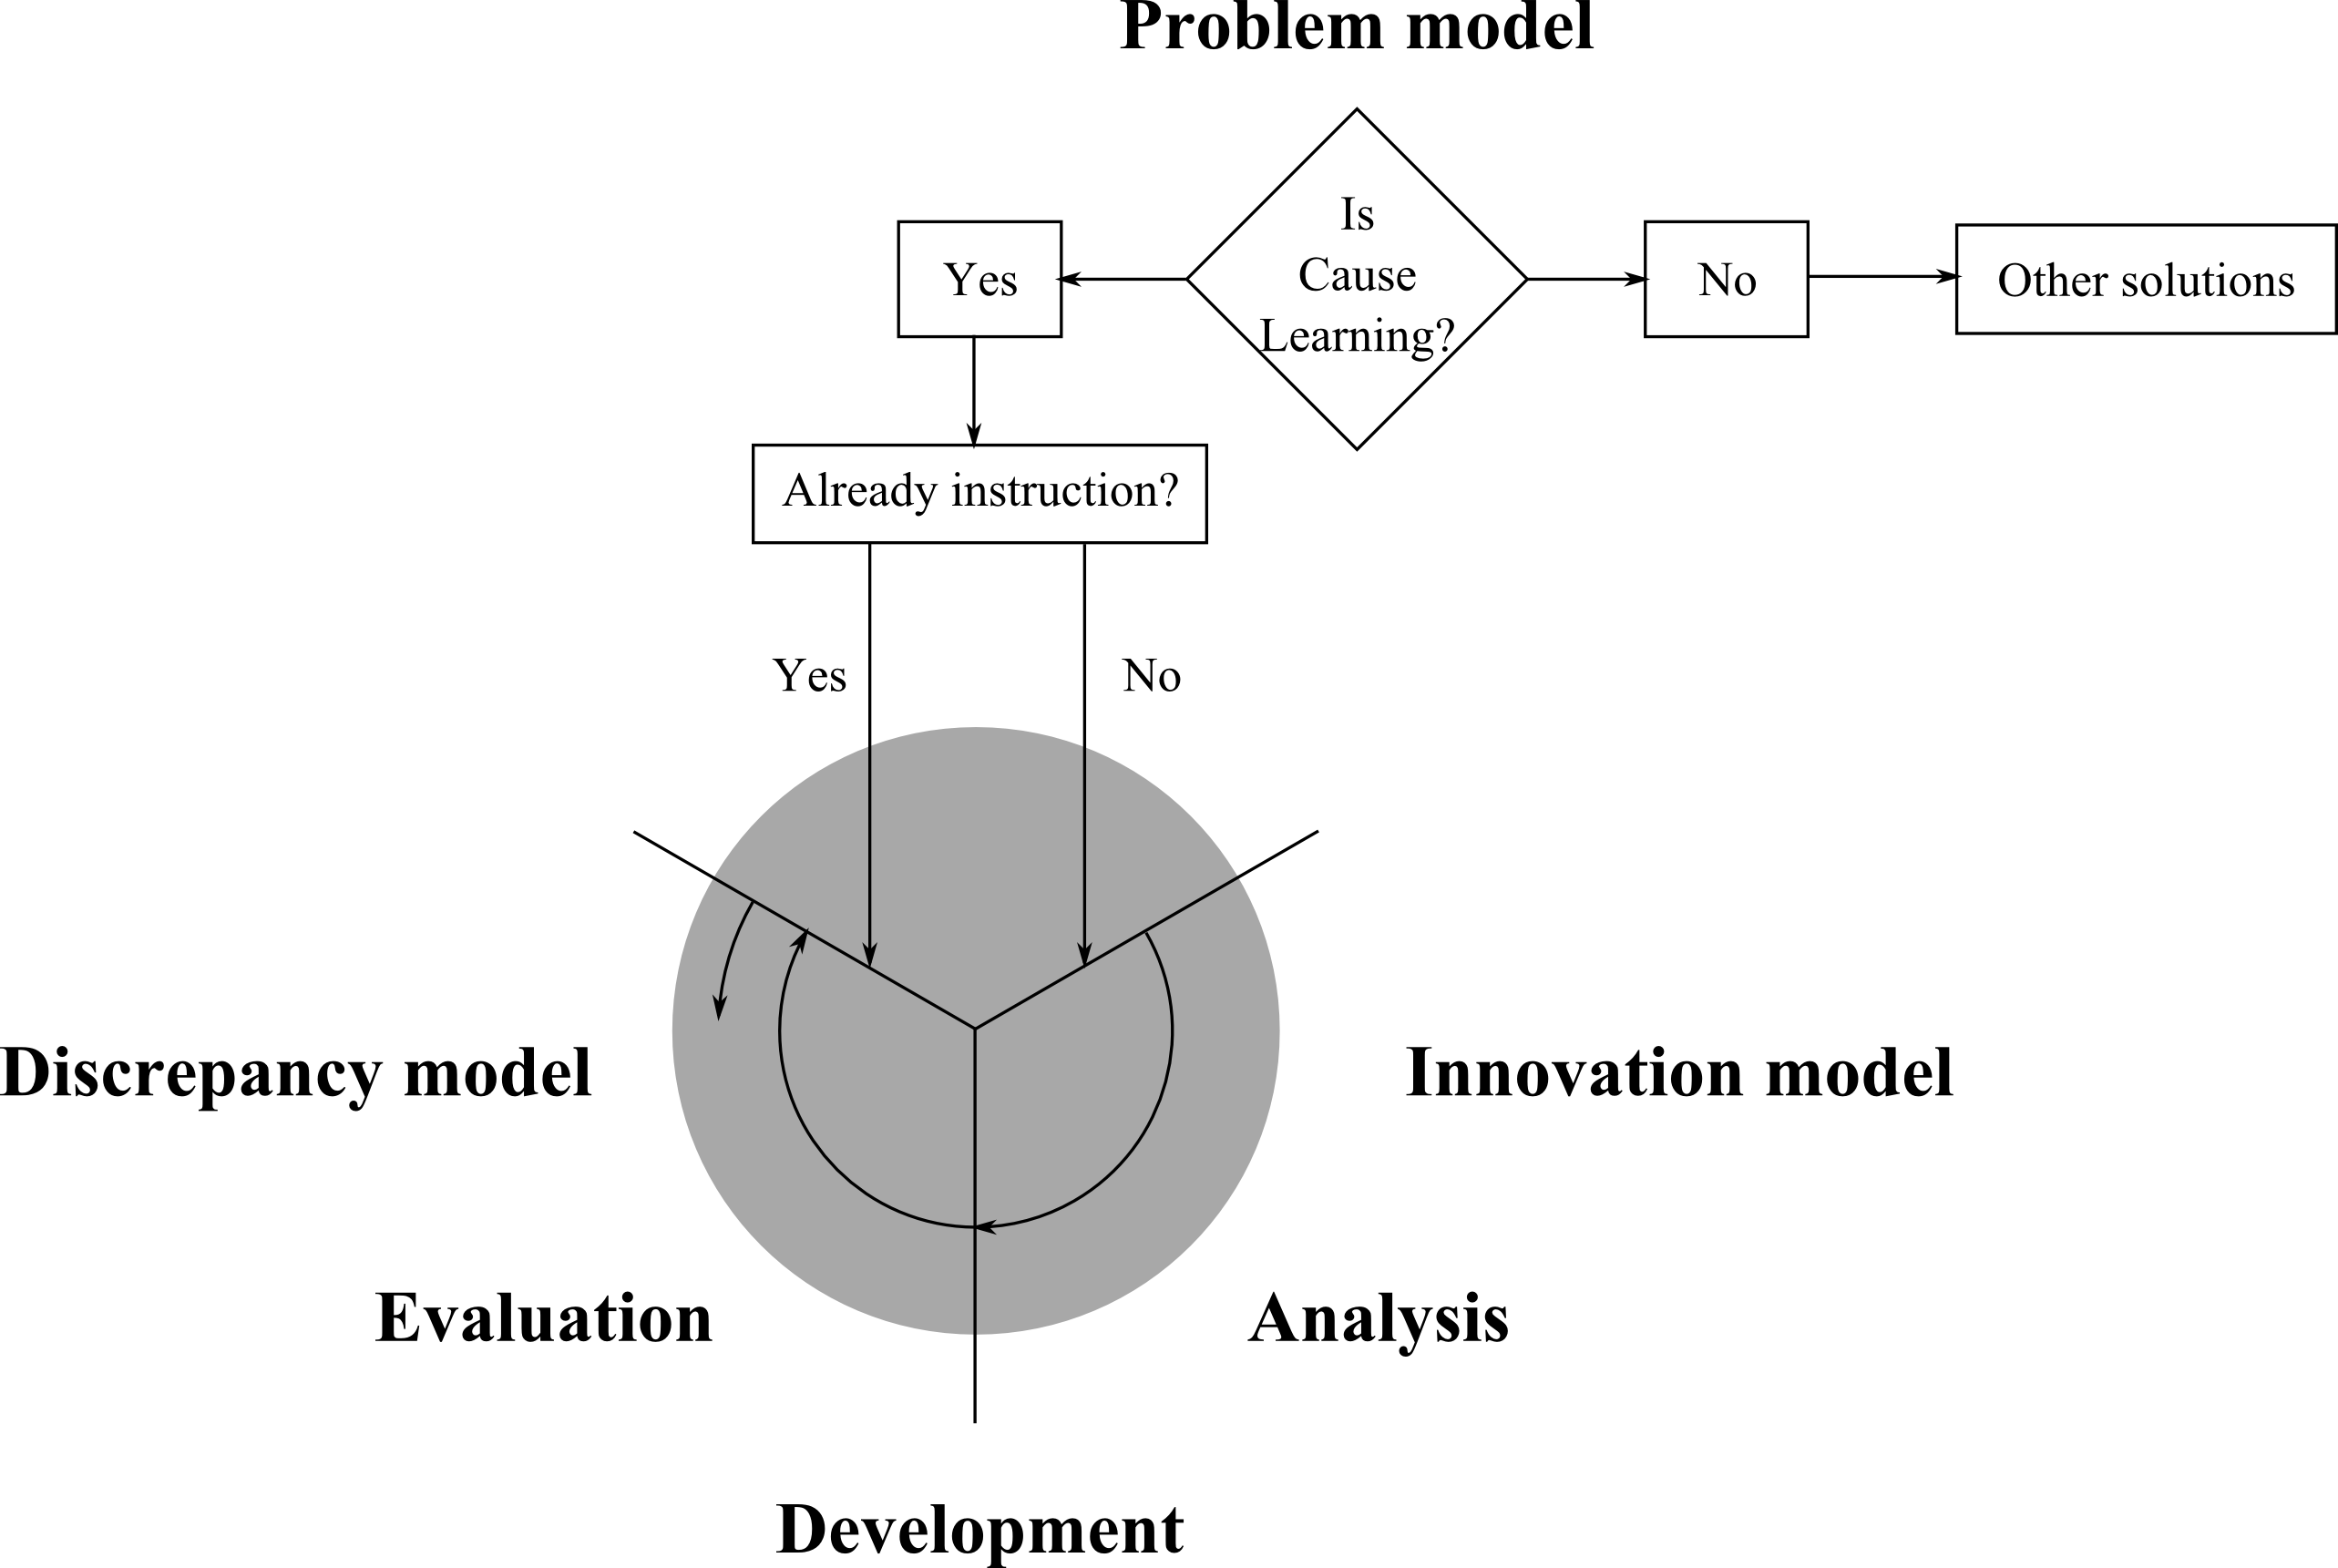
\includegraphics[width=\textwidth]{img/needsassessment.png}
    \caption{The three sides of needs assessment \protect\cite{instructionaldesign}}
    \label{fig:needsassessment}
\end{figure}

As can be seen in figure~\ref{fig:needsassessment}, the discrepancy model for needs assessment uses evaluative methods rather than analytical in order to establish the needs within the organisation. These methods include establishing the goals of the instructional system, determining how well these goals are currently being achieved, determining the gaps, prioritising the gaps, and determining which gaps are instructional needs (or in this case, educational needs). These remaining gaps can consecutively be used as a basis for determining the general use cases of the educational product. Normally an instructional designer tries to come into the organisation as a tabula rasa, without any preconceptions on what he would want to achieve and merely try to solve the real problem apparent in the organisation itself. However, because this design is theory driven rather than problem driven, it was merely checked with the teacher whether the problems stated in literature are also a problem here.

The first step was to confirm whether the goal stated by \citeA{glaserfield} of wanting students to memorise many facts in a meaningful way. Upon prompting the teacher what she deemed to be most important for her students to take away from her lessons was for them to become more familiar with the Dutch Renaissance writers or work. For example, she stated that she wanted the students to at least recognise important names when they saw a street name such as the "P.C. Hooftstraat" or the "Vondelpark". She also would like the students to be able to distinguish between different genres of literature, such as the \emph{sonnet} or \emph{emblematiek}. Based on these statements, the goals within the context are in line with students memorising and understanding all of the facts, without them being too ambitious. There are also differences between her and the other two teachers, they namely only offered the materials presented within the books, whereas she offered some additional content which the students also needed to master. However, she also stated that she would be responsible for the extra materials, and that the tool could be only to learn the textbook materials. Finally, she provided a test from the previous year to offer some more concrete examples of what she wanted the students to know, of which an English translation is included in the appendix on page~\pageref{ch:exampletest}. From this test, more goals can be extrapolated, such as students having to not only distinguish different genres, but also to define them or provide characteristics, and recognise the application of these features in both examples of the time periods as well as modern examples. Furthermore, they have to be able to relate the famous writers and writings to the genres.

According to the teacher, the students were mostly able to score points on the reproduction questions, such as having them to provide definitions or enlisting characteristics of genres. Thereby, most students were able to (barely) pass the test, which was already regarded as an important achievement, however minimal it might be. In this regard, the teachers already had scaled down their expectations of the students quite a bit to a realistic and feasible bar. The teacher also tried to make the material more appealing by focusing on examples, with succes.

However, as already indicated before, the main problem of students learning just before the exam and then forgetting about it remained an issue for the teacher, and more improvements could be made towards creating an understanding of the content by the students. Furthermore, although the examples make the content more appealing, according to the teacher students generally still did not experience the topic of Dutch renaissance literature as engaging or interesting (see also \citeNP{heemskerk}). Finally, most of the students would rapidly forget what they have learned after the exam, which the teacher did experience as wasteful. Therefore, the general categories of improvement can be enlisted as the students insufficiently understanding the content, not being immersed or engaged with the content (adequately), and retaining the acquired knowledge for a too short period of time.

Within the context of the Flashmap system, for now only the insufficient comprehension and retention of the content are prioritised, since there is no real evidence within the studied literature that the tool would also make content more immersive (although this could still be a side effect of the tool). These gaps are both instructional needs and are therefore appropriate gaps to tackle within the design.

\subsection{The learning environment}

Although \citeA{instructionaldesign} do enlist some of the steps necessary for describing the learning environment, \citeA{curricularspiderweb} provides a more widely used and thorough model, and therefore this will be used instead. This model is depicted in figure~\ref{fig:spiderweb}, and displays the relevant components which have to be taken into account for implementation of educational innovations. They are arranged as a spider's web, nog only illustrating their many inter-connections, but also underlining the vulnerability of the whole implementation. These aspects will be visited one by one from the perspective on the school, since the learner will be addressed separately in the next section.

\begin{figure}
    \centering
    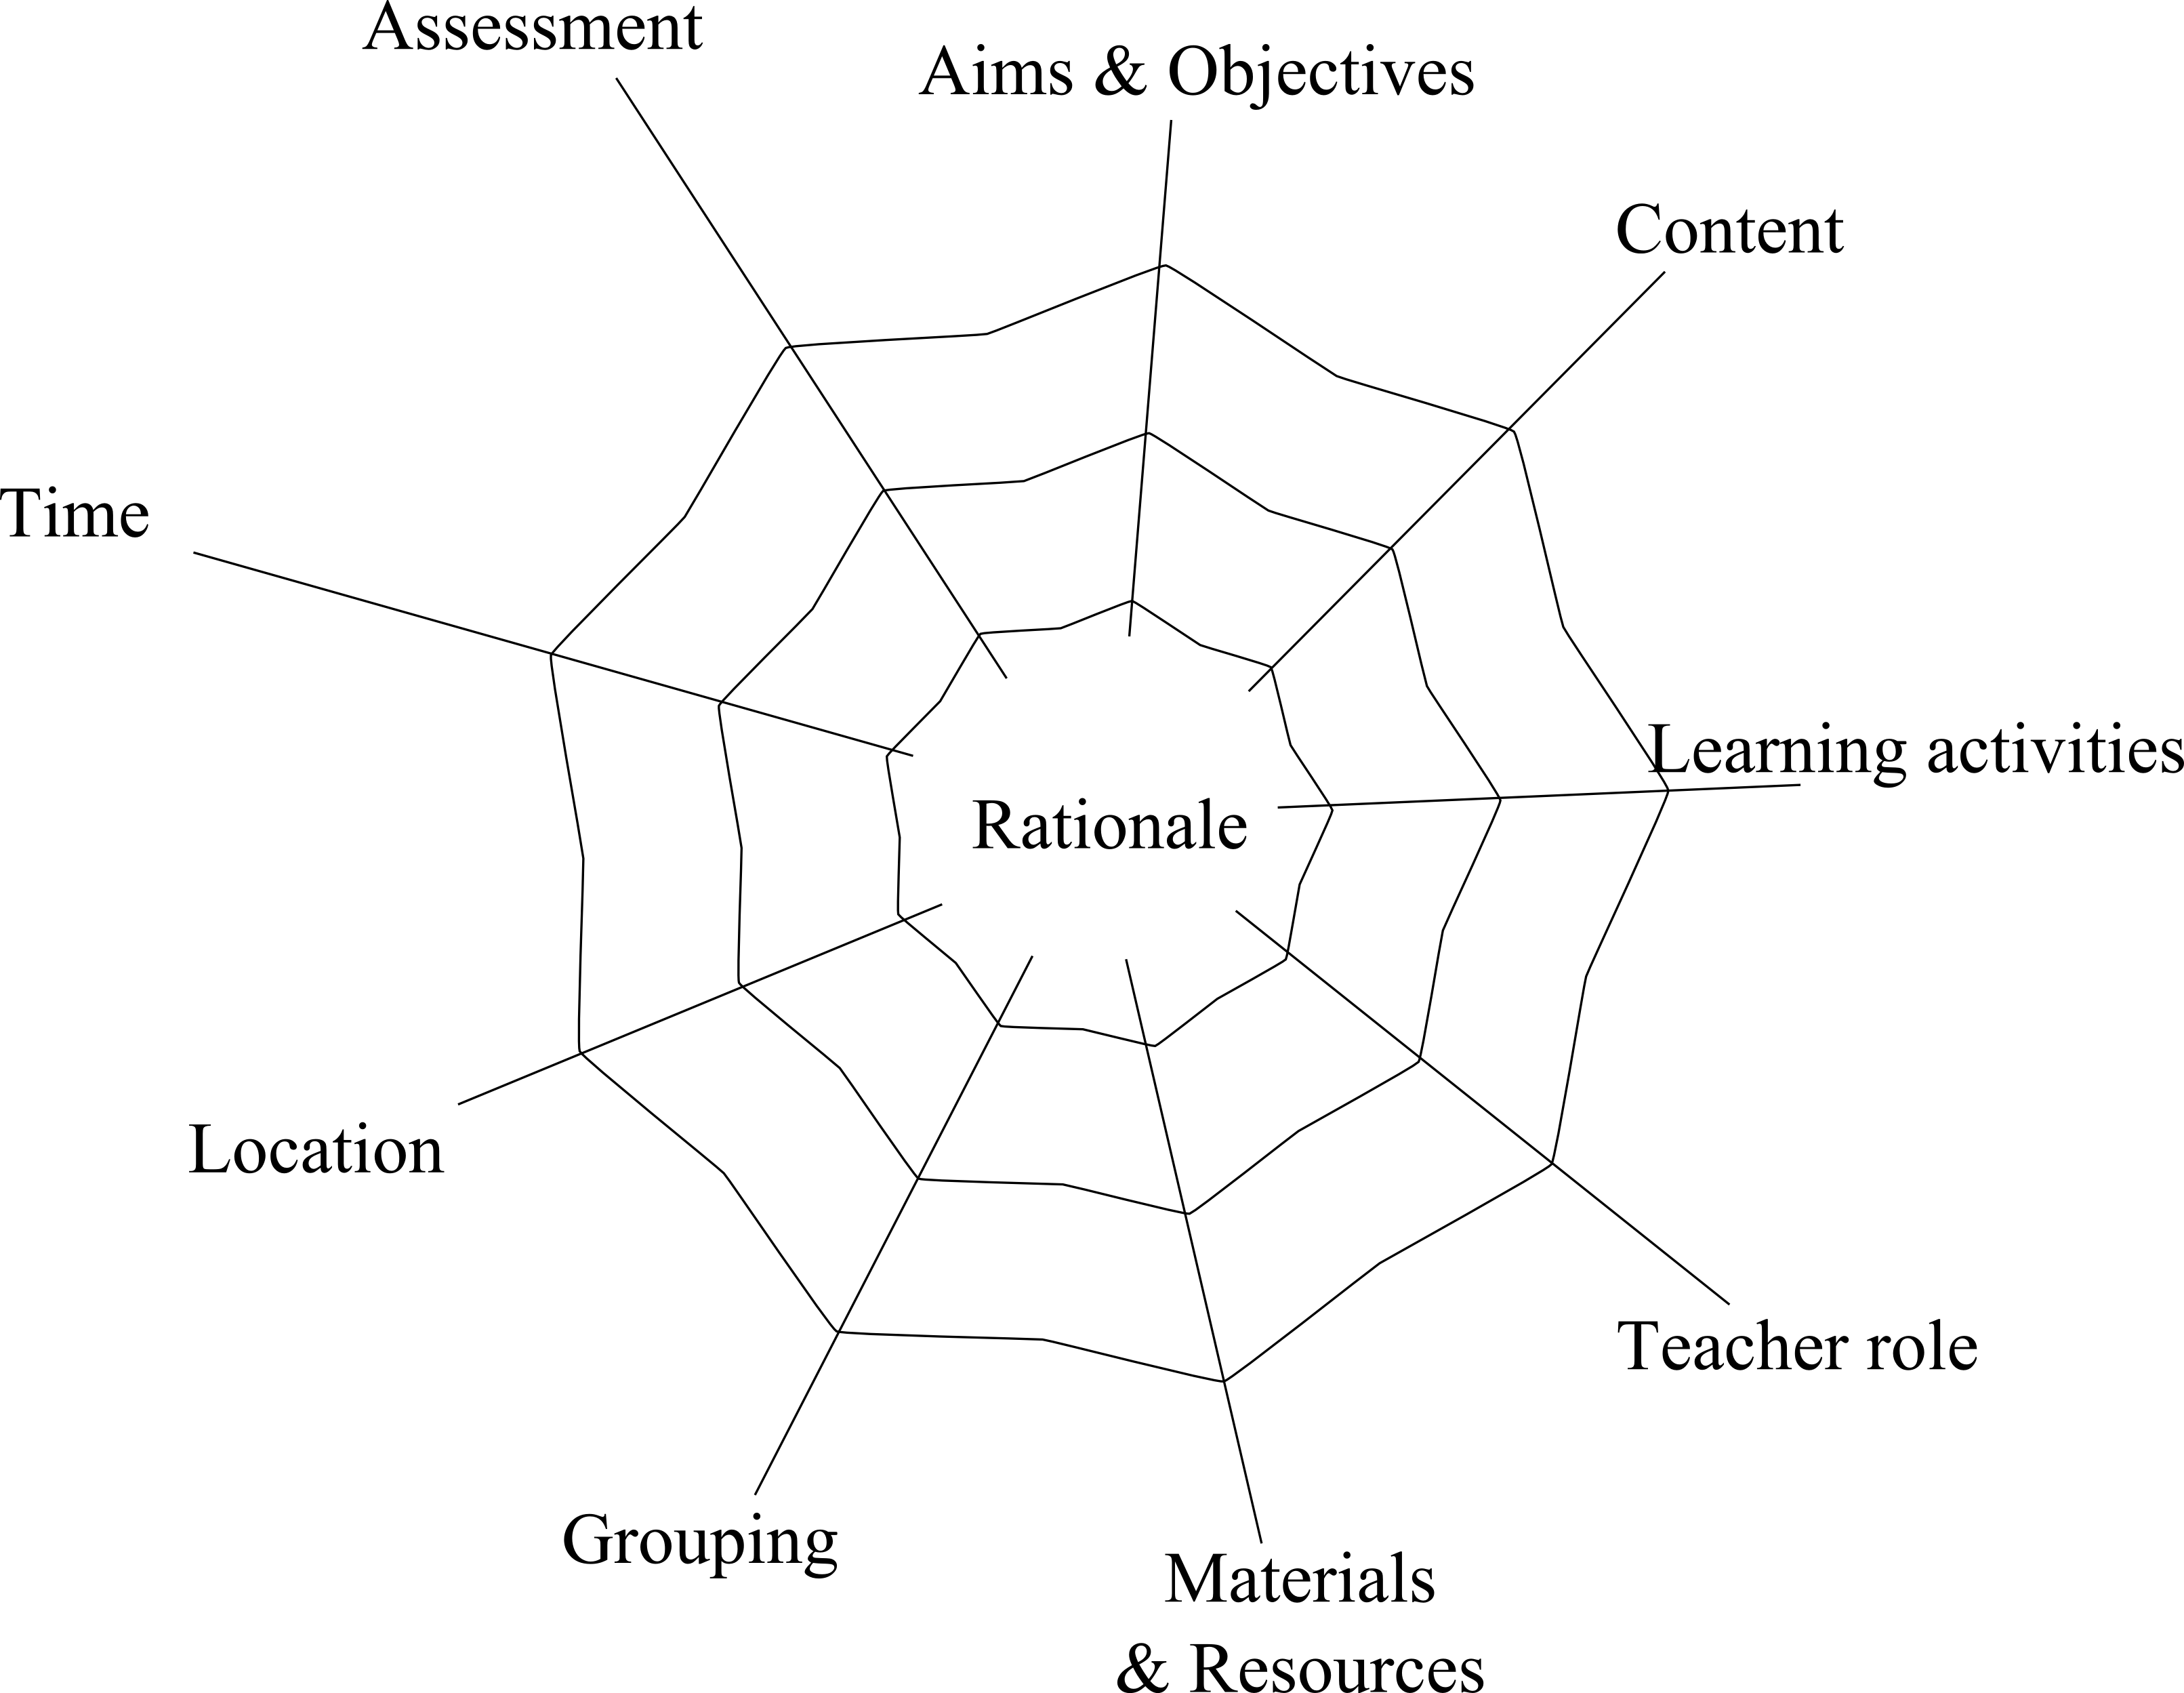
\includegraphics[width=0.7\textwidth]{img/curricular_spiderweb.png}
    \caption{The curricular spiderweb \protect\cite{curricularspiderweb}}
    \label{fig:spiderweb}
\end{figure}

The central aspect, \emph{rationale} (or vision), represents the question why students are learning the content in the first place. From the previously visited educational philosophies, one could make many arguments why students should familiarise themselves with Dutch renaissance literature: from a perennialistic or essentialistic perspective one could argue that it is the only way this knowledge can be transferred to the next generation and keeping it relevant; a progressivist could argue that one should first be familiar with older genres before one improve upon them or create new genres; reconstructivists might deem it important since it explains something about the national heritage, and thereby point out the flaws of the old ways; and finally an existentialist sees art in general as a meaningful way for self discovery. This intrinsic motivation is heavily dependent on the individual motivations and philosophy of the teacher. Most of these arguments are represented in diverse Dutch opinion pieces (e.g. \citeNP{opinion1, opinion2}). In the case of the consulted teacher, the arguments provided seemed to come mainly from the perennialistic and essentialistic perspective, namely that the content is part of our cultural identity and thereby important \emph{an sich}. However, she also indicated the existentialist self-discovery to be valuable. Furthermore, schools are extrinsically motivated to teach the material, since it has to demonstrate to society (mainly the exam committee) that their students have mastered this content. This is mainly related to subdomain E2 and E3 in the Dutch national exam programm, which states that a student can recognise and distinct between literary textgenres, and apply literary concepts in the interpretation of literary work; and that a student can provide the outlines of the (Dutch) literature history, and place literary works in this historical perspective.

Both the content and aims \& goals are already stated in the needs assessment, and can be summarised as: Students have to learn about prominent writers and genres within the context of Dutch renaissance literature; and have to be able to recognise important names and concepts, be able to define them or relate them to each other, and apply features of genres in examples of texts.

The course consists of two different types of learning activities, which are classroom instruction, and individual learning at home by the students. Their are two sessions of classroom instruction, both lasting 50 minutes, in which the 100 students are divided over the three teachers in static groups on separate locations. These lessons take place over the course of two weeks, with one lesson provided in one week. Within these lessons, the teachers transfer knowledge and provide excersises for the students. Outside of the lessons, the students still have to study the textbook Laagland individually \cite{laagland}, which contains all of the materials which will be prompted on a final written assessment. As already stated before, the teacher indicated this activity mostly to take place on the evening before the assessment, and only on a superficial level. Finally, this assessment takes place in the second week after the final instruction, and will be similar to the example test included in the appendix on page~\ref{ch:exampletest}.

The teacher stated that the course mainly consisted of the rote memorisation of facts, and that she was still doubtful whether the students would actually be willing to participate in the evaluation of the Flashmap system. Yet, she did see the general use of the tool for achieving the learning goals, and therefore still seemed to be enthusiastic in cooperation and encouraging the students to participate. The only two technical problems are that there is not too much time for extra activities within the lesson plan and the teachers being quite busy themselves, and that the technological possibilities within the classroom are limited. Within the classroom, only a couple of computers are available for use, and still run relatively old software. Therefore, the activities envolved in using the flashmap have to target the individual learning of students, since they have more time outside of the lesson plan, and mostly do possess the hardware and software necessary to run the software.

\section{Analysis of the learner}



\subsection{Four categories of learner characteristics}

\citeA{instructionaldesign} propose a methodology for assessing a learner which focuses on two axes: Stable and Changing, and Similarities and Differences, creating 4 categories. Within these categories, different types of learner characteristics, which are enlisted in table~\ref{tab:catslearner}. Stable similarities involve characteristics which are similar among people and do not change over time, such as sensory capabilities and their corresponding perceptual responses, the way people process information (as described in the \nameref{ch:theory} on page~\pageref{ch:theory} for example), and finally the ways and conditions in which people learn. Stable differences relate to characteristics different among people but stable over time, such as certain aptitudes, cognitive styles, psychosocial traits, or inheritary traits such as gender, ethnicity \& racial group. Changing similarities are similarities that do change over time, these characteristics are mainly attributed towards development processes. Finally, changing differences are differences in development accross people, which can mainly be attributed towards different upbringings or interests. Instead of visiting the learner characteristic according to each above mentioned category, \citeA{instructionaldesign} propose an more conveniently arranged outline which will be used in the next sections.

\begin{table}[hb]
\centering
\begin{tabular}{l|l|l|}
         & Similarities                                                                                                                      & Differences                                                                                                                        \\ \hline
Stable   & \begin{tabular}[c]{@{}l@{}}Sensory Capacities\\ Information processing\\ Types and conditions of learning\end{tabular}            & \begin{tabular}[c]{@{}l@{}}Aptitudes\\ Cognitive Styles\\ Psychosocial traits\\ Gender, Ethnicity, \& Racial Group\end{tabular}    \\ \hline
Changing & \begin{tabular}[c]{@{}l@{}}Development Processes:\\ - Intellectual\\ - Language\\ - Psychosocial\\ - Moral\\ - Other\end{tabular} & \begin{tabular}[c]{@{}l@{}}Developmental state:\\ - Intellectual\\ - Other\\ Prior learning:\\ - General\\ - Specific\end{tabular} \\ \hline
\end{tabular}
\caption{The four categories of learner characteristics \protect\cite{instructionaldesign}}
\label{tab:catslearner}
\end{table}

\subsection{Cognitive characteristics}

\subsection{Physiological characteristics}

\subsection{Affective characteristics}

\subsection{Social characteristics}

% Stable similarities:
%   Described in the cognitive theory chapter
% Stable differences:
%   About the same intelligence level (vwo), but still individual differences
%   Different cultural heritages: religions (atheism, christianity (reformed and catholic), islam, other), ethnicities (and therefore interests and prior knowledge)
%   Different chosen subjects: atheneum vs gymnasium, culture vs nature (and therefore interests and aptitutes)
%   Locus of control
% Changing similarities:
%   Discipline and motivation
% Changing differences:
%   Different cultural heritages: religions (atheism, christianity (reformed and catholic), islam, other), ethnicities (and therefore interests and prior knowledge)
%   Different chosen subjects: atheneum vs gymnasium, culture vs nature (and therefore interests and aptitutes)
% How to relate this framework with a personal framework?
%   How is this done in the textbook

% Maybe use the outline at the end of the chapter instead for the structure

\section{Analysis of the task}

% Description of the different sections within the textbook, and reference to the concept mapping design chapter
